\section[Effects on downstream analysis]{Effects on downstream analysis - not quite the missing link, but close}
\label{variantcalling-sec:downstream}

The ability to find additional shared variants has significant impact on our understanding of cancer evolution and the timing of initiation and metastatic seeding. Recent work has shown, that similar to the well known genetic heterogeneity, there is heterogeneity when it comes to metastatic seeding. While traditionally it was thought that tumours only metastesised after they reached a certain size, to escape the restrictions of the niche, like reduced nutrition, recent publications showed, there is also very early metastatic seeding \cite{Hu2019}. 
But all those methods are ultimately based on the somatic variants found in the data, so if we improve on the input of the downstream analysis methods, we can expect a clearer and possibly more granular result.

In this section I will highlight for a few examples on how big the effect can be for methods, like phylogenetic reconstruction and clonal decomposition, which use somatic variants as input.

\subsection[Polygenetic reconstruction]{Phylogenetic reconstruction}
\label{variantcalling-sec:phylo}
As this work is not about the advantages and shortcomings of different phylogenetics reconstruction tools, we will not show a comprehensive amount of these tools, but rather focus on the results.  For this reason, we chose to use neighbour joining (NJ) \cite{Saitou1987}, because it is fast, readily available in most phylogenetic reconstruction toolkits and if the input distance is correct, the output will be correct. And even, if the distance is not 100\% correct, if the distance is ``nearly additive`` and the input distances are not far off the real distance, the tree topology will still be reconstructed correctly \cite{Mihaescu2007}. Lastly, in contrast to many other methods like UPGMA and WPGMA \cite{Sokal1958}, NJ does not assume an equal mutation rate of each sample, because we know, that the molecular clock hypothesis \cite{Zuckerkandl1962} is not valid for different lineages of cancers \cite{Shibata2010}.

While there are lots of distance measures for DNA sequences, which allow accounting for different probabilities of transitions and transversions as well as uneven base composition, models like F81 \cite{Felsenstein1981} or HKY85 \cite{Hasegawa1985} are only really designed for germline mutations and are not easily applicable for subclonal somatic mutations, which is why we decided to first transform the variants present in all samples into a binary occurrence vector and then calculating the Hamming distance \cite{Hamming1950} between all samples. This generates a maximum parsimony approach and the branch length of the trees will be directly translatable to the amount of variants which are different between samples. 

\autoref{fig:ca99phylo} shows both the reconstructed phylogenies when using the variants found with the default tumour-normal method and our improved joint method and using the exact same reconstruction method otherwise.

\begin{figure}[!ht]
\centering
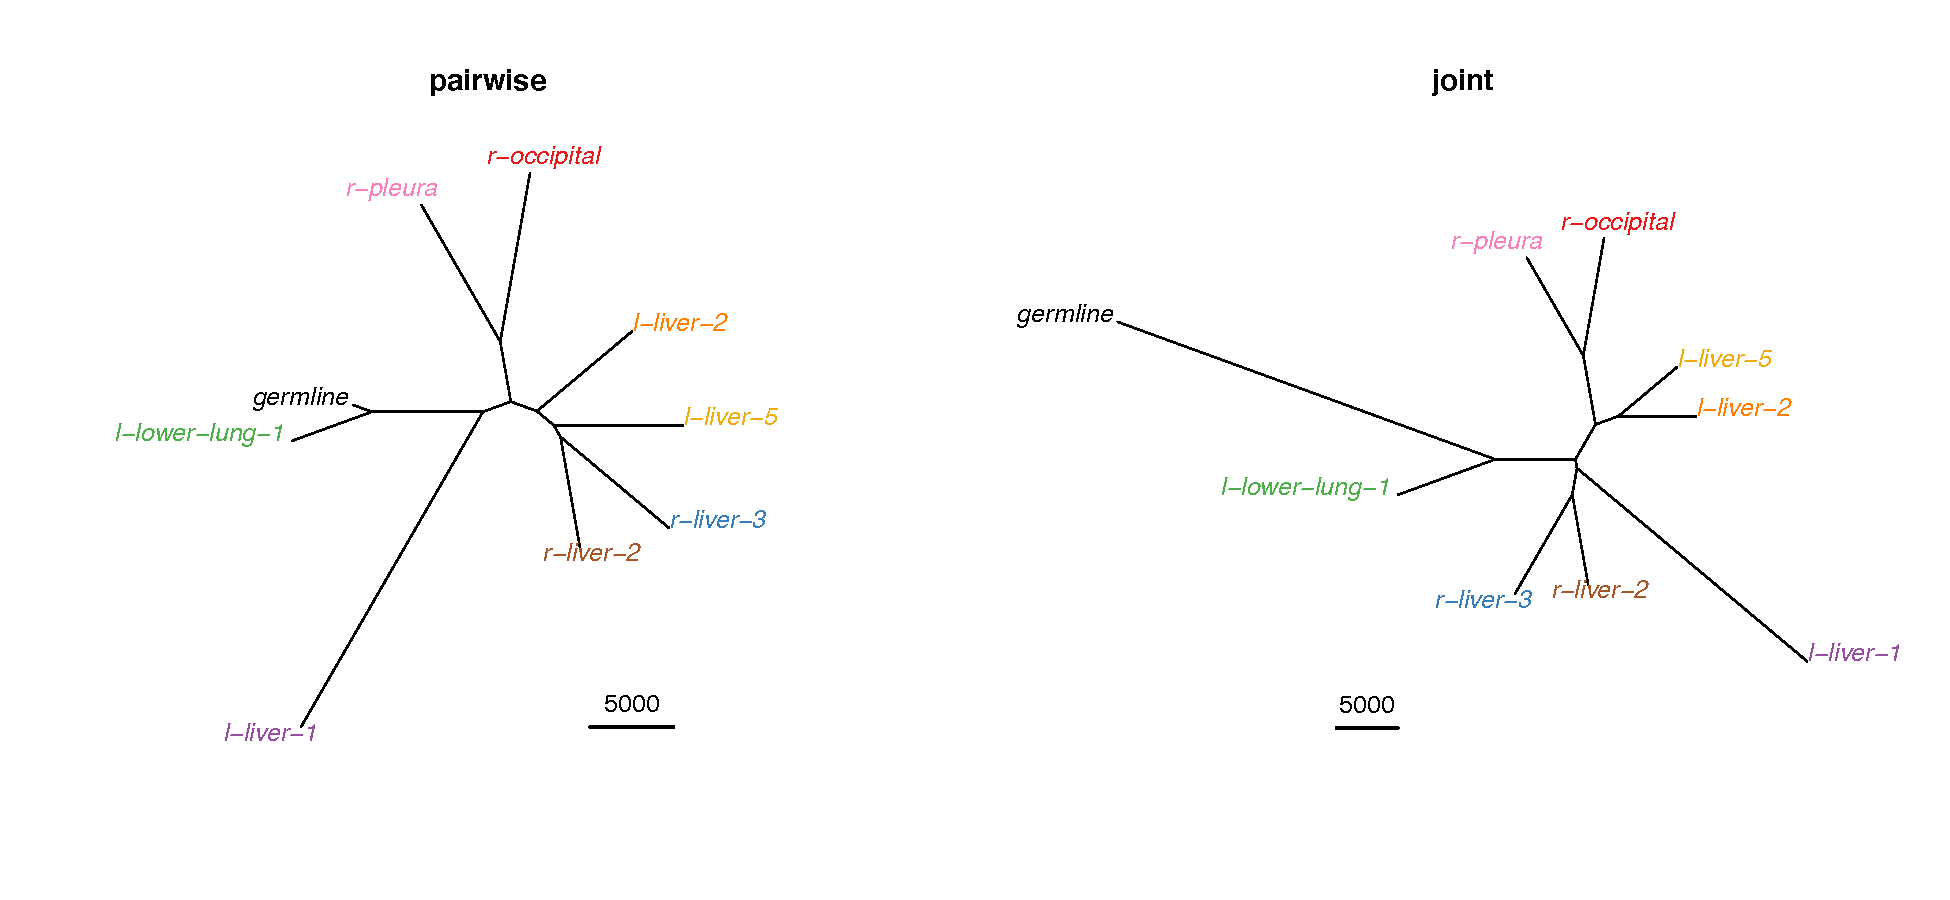
\includegraphics[width=.99\linewidth]{Figures/phyloCA99.pdf}
\caption[Reconstructed phylogenies of joint samples]{Reconstructed phylogenies of a patient with multiple spatially distinct samples; Reconstruction method is neighbour joining for both cases, only the input of the called variants is different. Tip labels describe the location of the sample in the patient. Trees are shown as unrooted with germline as fixated origin point; black line ruler shows the length of an edge with 5000 mutations}\label{fig:ca99phylo}
\end{figure}

There are several obvious changes, first, the longer edge connecting the the germline, which we consider as the state of no somatic variants, to all other samples. This shows that there are many more shared mutations in all samples, than what would have been anticipated with the default method. As the accumulation of somatic variants is still used as a proxy for timing and cell divisions, when assuming a high mutation rate for lung cancer ($5.3 \cdot 10^{-8}$ from \citeauthor*{Werner2020} \cite{Werner2020}) this difference of $\approx 36000$ variants is equivalent to $\approx 2000$ cell divisions. While the cell doubling rate of lung cancers is highly dependent on the type \cite{Arai1994}, this difference makes a huge difference when assessing the timing of the tumour initiation and further evolution. 

Secondly, there have been topological changes, which generate a bifuricating edge between the warm coloured pleura, occipital, l-liver-2 and l-liver-5 samples, which fits significantly better with the clinical history and PET scans of the patient, as these are the sites of progression, which lead to the death of the patient in contrast to the earlier sites of disease.

\autoref{fig:tanglePhyloCa99} shows a topology focused view of the two trees, which highlights the breaks which are needed to morph one tree into the other with dotted edges \cite{Vienne2018}. The common subtrees are coloured the same on both sides and connecting lines show identical labels. This format shows that while the trees look quite similar at first glance, they show vastly different topologies.

\begin{figure}[!ht]
\centering
\includegraphics[width=.99\linewidth]{Figures/tanglePhyloCA99.pdf}
\caption[Tanglegram of the reconstructed phylogenies]{Side by side view of the reconstructed trees from \autoref{fig:ca99phylo}; internal edges, which are distinct between trees are shown as dotted lines; common subtrees are shown in red and green; Tree labels have been sorted to minimise distance between labels; axis show the hamming distance between two nodes. Visualisation generated with dendextend \cite{Galili2015}}\label{fig:tanglePhyloCa99}
\end{figure}

One example of this is ``l-liver-3`` which was a singleton, almost an outlier, in the pairwise reconstructed tree but is clustered together with ``r-liver-2`` and ``r-liver-3``. Generally, there have been additional changes, which make the topology more granular. Where all of the ``l-liver-*`` samples were shown as an almost linear branching off the main stem, they are now further subdivided and each show distinct mutations, like ``l-liver-2`` and ``l-liver-5`` (\autoref{fig:tanglePhyloCa99}).

\todo[color=orange, inline]{show before vs after for phylogenetic reconstruction}


\subsection[Clonal deconvolution]{Clonal deconvolution}
\label{variantcalling-sec:clonal}

\todo[color=orange, inline]{show before vs after for clonal deconvolution}